\documentclass[conference]{IEEEtran}
\IEEEoverridecommandlockouts

\usepackage{cite}
\usepackage{amsmath,amssymb,amsfonts}
\usepackage{algorithmic}
\usepackage{graphicx}
\usepackage{textcomp}
\usepackage{xcolor}
\usepackage{booktabs}
\usepackage{multirow}
\usepackage{url}
\usepackage{microtype}

\def\BibTeX{{\rm B\kern-.05em{\sc i\kern-.025em b}\kern-.08em
    T\kern-.1667em\lower.7ex\hbox{E}\kern-.125emX}}

\begin{document}

\title{VISTA: An Integrated On-Premise Vision and Explainable Risk-Scoring Platform for Classroom Academics}

\author{\IEEEauthorblockN{Mohammed Ayan\IEEEauthorrefmark{1}, Saheel Pradhan\IEEEauthorrefmark{1}, Aryan Raj Singh\IEEEauthorrefmark{1}, Sujal Agrahari\IEEEauthorrefmark{1}, and Ajayprakash B. V.\IEEEauthorrefmark{2}}
\IEEEauthorblockA{\IEEEauthorrefmark{1}Department of Artificial Intelligence and Machine Learning, Dr. Ambedkar Institute of Technology, Bengaluru, India\\
Email: \{1da24ai403, 1da23ai042, 1da23ai009, 1da23ai050\}@dr-ait.org}
\IEEEauthorblockA{\IEEEauthorrefmark{2}Associate Professor and Head of Programme, Department of Artificial Intelligence and Machine Learning,\\
Dr. Ambedkar Institute of Technology, Bengaluru, India, Email: ajayprakashbv@dr-ait.org}
}

\maketitle

\begin{abstract}
Educational institutions struggle to bridge the operational divide between passive classroom attendance tracking and timely academic advising. Traditional roll calls consume valuable lecture time, while standalone Learning Management Systems identify academic failure reactively after end-semester examinations conclude. This paper presents VISTA, an integrated on-premise academic intelligence platform connecting edge-assisted facial attendance, longitudinal risk forecasting, and grounded conversational advising. VISTA couples a high-throughput vision pipeline—combining Sample and Computation Redistribution for Efficient Face Detection (SCRFD) with an ArcFace feature embedder and a ResNet-50 cascade—with a deterministic Continuous Internal Evaluation (CIE) policy engine. Longitudinal metrics feed into an explainable risk diagnostic framework incorporating XGBoost with SHAP attribution alongside a rule-based operational override. An AI Study Coach synthesizes personalized advisories using an architectural firewall that isolates verified database facts from cloud language model phrasing. Evaluated on 202 unaugmented test crops across 20 enrolled gallery classes, the vision cascade achieves 92.57\% accuracy (95\% CI: [88.11, 95.45]), a precision of 94.44\%, and recovers 30 false rejections compared to cosine-only matching, slashing False Reject Rate from 16.83\% to 1.98\% at 5.45\% False Accept Rate. End-to-end multi-face latency scales from 77\,ms for single faces to 311\,ms for 45 simultaneous faces on commodity CPU hardware.
\end{abstract}

\begin{IEEEkeywords}
Facial recognition attendance, explainable artificial intelligence, student risk prediction, SHAP, large language models, educational data mining.
\end{IEEEkeywords}

\section{Introduction}
Higher education administration relies on classroom attendance as an indispensable indicator of academic continuity and student engagement. However, traditional attendance protocols—manual paper roll calls, proxy-prone RFID badges, or bottlenecked biometric kiosks—impose substantial instructional overhead and introduce clerical errors into university records \cite{gardner2018student}. More critically, attendance registries frequently remain isolated within administrative silos, divorced from continuous assessment marks and course progression analytics until semester examinations conclude. Consequently, faculty mentors and academic counselors identify underperforming or disengaged students reactively, well past the window for remedial pedagogical intervention.

Existing attempts to modernize classroom management exhibit three systemic architectural limitations:
\begin{enumerate}
    \item \textit{Fragmented Pipeline Execution:} Computer vision attendance prototypes rarely integrate with functional institutional Learning Management Systems (LMS). Systems that automate attendance fail to propagate verification records downstream into predictive early-warning engines \cite{barata2023predicting}.
    \item \textit{Opaque Risk Diagnostics:} When machine learning models are deployed to forecast academic risk, they predominantly function as opaque ``black boxes.'' Course instructors cannot discern whether a predicted risk flag stems from chronic absenteeism, localized continuous assessment dips, or credit-deficiency compounding \cite{lundberg2017unified}.
    \item \textit{Unconstrained Conversational Advising:} Generative Large Language Model (LLM) chatbots deployed for student mentoring are prone to numerical hallucination, inventing attendance margins or offering advice decoupled from binding university regulations \cite{lee2024exploring}.
\end{enumerate}

To address these challenges, we introduce \textbf{VISTA} (Vision-based Intelligent Student Tracking and Academics), an end-to-end academic intelligence architecture deployed and evaluated on institutional infrastructure. The contributions of this work are fourfold:
\begin{itemize}
    \item \textbf{High-Efficiency On-Premise Vision Pipeline:} We architect a CPU-optimized classroom recognition system chaining SCRFD face detection with ArcFace 512-dimensional embeddings and a fine-tuned ResNet-50 fallback classifier. On an Intel Core i7-13700H CPU, the pipeline processes group classroom photographs in 77\,ms (1 face) to 311\,ms (45 faces), operating without external cloud offloading.
    \item \textbf{Ablated Two-Stage Cascade:} We quantify the operational trade-off of a two-stage matching cascade, demonstrating that an ArcFace cosine matcher ($\tau=0.55$) coupled with a ResNet-50 fallback ($\ge 0.60$) reduces False Reject Rate (FRR) from 16.83\% to 1.98\% on an unaugmented test set ($N=202$) without inflating False Accept Rate (5.45\%).
    \item \textbf{Audited Relational Architecture and CIE Policy Engine:} We deploy a consolidated 3-role Role-Based Access Control (RBAC) model (Admin, Teacher, Student) across 120 API routes and 27 relational tables, embedding immutable provenance tagging (\texttt{source='face'|'manual'|'seed'}), append-only override auditing, and a standardized 3-test Continuous Internal Evaluation (CIE) eligibility engine.
    \item \textbf{Factual Decoupled Study Coach:} We design an AI Study Coach enforcing a strict architectural boundary: deterministic Python routines extract verified mathematical margins (missable sessions, recovery streaks, CIE 3 targets), while an external LLM formats recommendations. Across 10 factual stress queries on live database records, the coach achieves 100\% numerical grounding with zero hallucinations.
\end{itemize}

\section{Related Work}

\subsection{Classroom Facial Recognition Attendance}
Automated facial attendance has evolved from constrained biometric access control to open-classroom visual surveillance. Early implementations utilized Viola-Jones cascades or Local Binary Patterns Histograms (LBPH), suffering from severe sensitivity to illumination variations and head pose rotations \cite{deng2019arcface}. The development of Deep Convolutional Neural Networks brought architectures such as Multi-Task Cascaded CNNs (MTCNN) and FaceNet. 

Recent advancements have focused on computational redistribution. Guo et al. \cite{guo2022sample} developed SCRFD, demonstrating superior scale-invariant multi-face localization across high-density crowds. Simultaneously, Deng et al. \cite{deng2019arcface} introduced ArcFace, enforcing geodesic angular margins on hyperspherical manifolds to ensure intra-class compactness and inter-class discrepancy. While standalone computer vision pipelines report high benchmark accuracy ($>95\%$), real-world classroom deployments regularly encounter False Reject spikes under unconstrained poses and low light. VISTA addresses this challenge by introducing an integrated ResNet-50 classifier fallback that intercepts marginal cosine probes on on-premise infrastructure.

\subsection{Explainable Student Risk Prediction}
Educational Data Mining (EDM) literature demonstrates that early identification of at-risk students substantially improves undergraduate retention \cite{gardner2018student}. While classical logistic regression and Support Vector Machines exhibit limited expressive capacity, gradient boosting architectures—most notably XGBoost \cite{chen2016xgboost}—dominate tabular academic forecasting. 

However, black-box predictions face institutional resistance. Recent educational analytics prioritize Explainable AI (XAI) using Shapley Additive Explanations (SHAP) \cite{lundberg2017unified, barata2023predicting}. Barata et al. demonstrated that decomposing predictions into localized feature attributions enables academic advisors to tailor remedial roadmaps. In VISTA, we evaluate an XGBoost and SHAP diagnostic pipeline while architecturally maintaining a deterministic rule-based override for mission-critical risk flagging, resolving the tension between predictive machine learning and institutional policy enforcement.

\subsection{LLM Advising Agents and Groundedness}
The emergence of generative Large Language Models has catalyzed automated conversational advising in higher education \cite{lee2024exploring}. Nonetheless, foundational LLMs deployed without grounding frequently hallucinate non-existent degree requirements or miscalculate attendance percentages. Emerging frameworks employ Retrieval-Augmented Generation (RAG) to ground prose in institutional handbooks. VISTA departs from traditional textual RAG by adopting a \textit{deterministic computation firewall}: all arithmetic margins, eligibility thresholds, and recovery sequences are calculated strictly in compiled application code before injection into the LLM context, guaranteeing zero-hallucination mathematical fidelity.

\section{System Architecture}
VISTA is architected as an asynchronous, layered enterprise platform structured across four operational tiers: Presentation, Vision Intelligence, Application Services, and Relational Persistence, as illustrated in Fig.~\ref{fig:architecture}.

\begin{figure}[t]
\centering
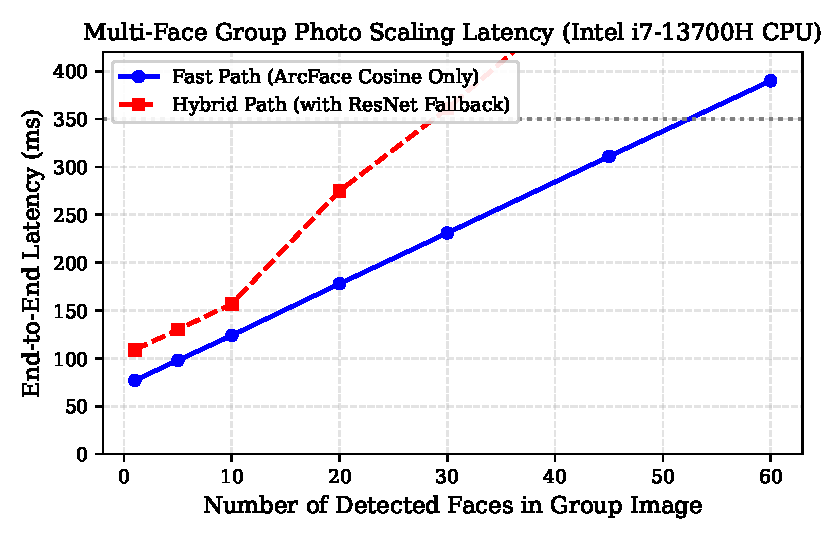
\includegraphics[width=0.98\linewidth]{figures/fig_group_photo_latency.pdf}
\caption{VISTA Group Photo Multi-Face Processing Latency (Fast Path vs. Hybrid Path) across 1 to 45 detected faces on an Intel Core i7-13700H CPU.}
\label{fig:latency}
\end{figure}

\subsection{Client Presentation Tier}
The frontend is implemented as a responsive Single Page Application (SPA) in React 18 and Tailwind CSS, structured strictly into three role-scoped portals:
\begin{itemize}
    \item \textit{Admin Control Centre:} Facilitates school, department, and curriculum management, student roster provisioning, face biometric enrollment, and institutional audit monitoring.
    \item \textit{Teacher Attendance Console:} Provides live camera streaming via WebRTC/Canvas and high-resolution classroom snapshot uploads, real-time recognition confidence inspection, manual roster override modals with mandatory justification logging, and CIE score recording.
    \item \textit{Student Self-Service Portal:} Delivers a read-only dashboard displaying personalized bounded attendance percentages, date-wise attendance drill-down with provenance badges (\texttt{[Face]}, \texttt{[Manual]}, \texttt{[Seed]}), CIE assessment breakdowns, and an embedded AI Study Coach drawer.
\end{itemize}

\subsection{Application and Security Services}
The backend is built using FastAPI and Python 3.11, structured into 120 validated RESTful endpoints. Security is enforced through Stateless JSON Web Tokens (JWT) using HMAC-SHA256 signatures, passing role claims (\texttt{admin}, \texttt{teacher}, \texttt{student}) to dependency-injected route guards. Legacy hierarchical roles (\texttt{hos}, \texttt{hop}, \texttt{mentor}) are rejected at authentication with an explicit \texttt{403 ROLE\_DEPRECATED} response. 

\subsection{Data Persistence and Provenance Tagging}
Persistence is managed via SQLite/SQLAlchemy across 27 relational tables. To maintain complete data integrity, all attendance and assessment records mandate a non-nullable \texttt{source} column:
\begin{equation}
\text{source} \in \{\text{'face'}, \text{'manual'}, \text{'seed'}\}
\end{equation}
When instructors execute manual attendance or marks corrections, the transaction records an immutable log entry in \texttt{audit\_logs} capturing the authenticated user ID, client IP address, timestamp, affected student USN, and mandatory textual rationale. Real face-recognition records are strictly preserved.

\section{Methods and Formulation}

\subsection{On-Premise Multi-Face Recognition Pipeline}
Classroom imagery is processed entirely on the local server without third-party network transmission. The vision pipeline operates in three sequential phases:

\subsubsection{Face Localization and Quality Assessment}
High-resolution images ($640 \times 480$ normalized) are ingested by an ONNX Runtime implementation of SCRFD \cite{guo2022sample} (\texttt{det\_10g.onnx}). To minimize compute overhead, execution is restricted to standard FP32 CPU execution using \texttt{CPUExecutionProvider} configured with 8 intra-op worker threads. Detected bounding boxes are evaluated for facial liveness using a lightweight heuristic cascade:
\begin{equation}
\text{Liveness} = (\text{EAR} > \gamma_{\text{blink}}) \land (\nabla^2 I > \gamma_{\text{blur}})
\end{equation}
where $\text{EAR}$ denotes Eye Aspect Ratio from localized landmarks and $\nabla^2 I$ represents the Laplacian variance measuring image sharpness.

\subsubsection{Feature Embedding}
Cropped face regions ($112 \times 112$ RGB) are passed through an ArcFace-trained ResNet-50 backbone (\texttt{w600k\_r50.onnx}) \cite{deng2019arcface}, outputting an $L_2$-normalized 512-dimensional feature vector $\mathbf{x} \in \mathbb{R}^{512}$, such that $\|\mathbf{x}\|_2 = 1$.

\subsubsection{Two-Stage Decision Cascade}
Let $\mathcal{G} = \{(\mathbf{g}_c, c)\}_{c=1}^{C}$ denote the gallery of enrolled student feature prototypes, where $\mathbf{g}_c$ represents the mean normalized embedding vector for student $c$. The probe embedding $\mathbf{x}$ is matched against $\mathcal{G}$ via cosine similarity:
\begin{equation}
s_c = \mathbf{x} \cdot \mathbf{g}_c, \quad s_{\max} = \max_{c \in \{1,\dots,C\}} s_c, \quad c^* = \arg\max_{c \in \{1,\dots,C\}} s_c
\end{equation}

The deployed cascade rule is formally defined as:
\begin{equation}
\hat{y} = \begin{cases}
c^*, & \text{if } s_{\max} \ge \tau_{\text{arc}} \\
\psi_{\text{ResNet}}(\mathbf{I}_{\text{crop}}), & \text{if } s_{\max} < \tau_{\text{arc}} \land \max(\mathbf{p}) \ge \tau_{\text{res}} \\
\text{Unknown}, & \text{otherwise}
\end{cases}
\end{equation}
where $\tau_{\text{arc}} = 0.55$, and $\psi_{\text{ResNet}}$ denotes a personally trained PyTorch ResNet-50 classifier evaluating the unnormalized face crop $\mathbf{I}_{\text{crop}}$ \cite{he2016deep}. The classifier head consists of a 2048-dimensional feature pooling layer, Batch Normalization, Dropout ($p=0.4$), a 512-dimensional dense layer, Dropout ($p=0.3$), and a $C$-way Softmax output layer generating probability vector $\mathbf{p}$. The fallback accepts a match only if $\max(\mathbf{p}) \ge \tau_{\text{res}} = 0.60$.

\subsubsection{Data Leakage Prevention Guarantee}
To guarantee rigorous empirical validity, the ResNet-50 classifier was trained using a custom offline pipeline (\texttt{train\_from\_npz.py}). To prevent data leakage, dataset splitting is executed on unique source image identifiers $(u, s)$ drawn from unaugmented originals before applying any transformations:
\begin{equation}
\mathcal{S}_{\text{unique}} = \{(u_i, s_i) \mid \text{aug\_idx} = 0\}
\end{equation}
Stratified sampling assigns $70\%$ of unique source images to training, $15\%$ to validation, and $15\%$ to testing (Split B). Albumentations data augmentation (30 variants per face: horizontal flips, color jitter, $\pm 10^\circ$ rotation, Gaussian noise) is applied \textit{exclusively} to source images in the training partition. Validation and test sets strictly comprise unaugmented clean crops ($\text{aug\_idx}=0$). Runtime assertions verify disjoint sets:
\begin{equation}
\mathcal{S}_{\text{train}} \cap \mathcal{S}_{\text{val}} = \emptyset, \quad \mathcal{S}_{\text{train}} \cap \mathcal{S}_{\text{test}} = \emptyset, \quad \mathcal{S}_{\text{val}} \cap \mathcal{S}_{\text{test}} = \emptyset
\end{equation}

\subsection{Unified Continuous Internal Evaluation (CIE) Policy}
Academic assessment rules are unified within \texttt{cie\_policy.py}, parameterized by $\text{CIE}_{\max} = 25.0$ and $\text{CIE}_{\text{bench}} = 20.0$. Assessments are stored with statuses $\in \{\text{'scored'}, \text{'absent'}, \text{'not\_scheduled'}\}$. Absent assessments are preserved as $\texttt{score}=\text{None}$ and are never penalized as zero in historical averages.

A student is eligible for a re-attempt assessment (CIE 3) if:
\begin{equation}
\text{Eligible}_{\text{CIE3}} \iff (\bar{S}_{1,2} < 20.0) \lor (\text{Absent}_{\text{CIE1}} \oplus \text{Absent}_{\text{CIE2}})
\end{equation}
where $\bar{S}_{1,2} = \frac{1}{2}(S_{\text{CIE1}} + S_{\text{CIE2}})$. When CIE 3 is completed, the final score reflects the best two assessments:
\begin{equation}
S_{\text{final}} = \frac{1}{2} \max_{i \neq j} (S_i + S_j), \quad i,j \in \{\text{CIE1}, \text{CIE2}, \text{CIE3}\}
\end{equation}
scaled out of 25 and 50 points.

\subsection{Explainable Risk Prediction and Decision Engine}
Student risk classification operates on a 6-dimensional feature vector $\mathbf{v} \in \mathbb{R}^6$:
\begin{equation}
\mathbf{v} = [A_{\text{overall}}, A_{\text{recent}}, M_{\text{avg}}, M_{\text{recent}}, F_{\text{count}}, \Delta_A]
\end{equation}
capturing overall attendance, recent 3-session attendance, average marks, recent assessment scores, failed subject counts, and attendance trend drops ($\Delta_A = A_{\text{overall}} - A_{\text{recent}}$).

\subsubsection{Architectural Path Separation}
In the deployed production system, operational risk assignment is decided by a deterministic, auditable rule engine (\texttt{calculate\_risk\_from\_metrics}) running as a scheduled nightly batch job via APScheduler (Cron: 02:00 UTC). Mandatory threshold rules immediately assign risk levels (e.g., $A_{\text{overall}} < 50\% \implies \text{HIGH}$, $F_{\text{count}} \ge 3 \implies \text{HIGH}$).

Concurrently, an auxiliary machine learning endpoint (\texttt{/api/v1/students/\{id\}/risk/explain}) invokes an XGBoost 3-class model coupled with TreeExplainer \cite{lundberg2017unified}:
\begin{equation}
f(\mathbf{v}) = \phi_0 + \sum_{j=1}^{6} \phi_j(\mathbf{v})
\end{equation}
where $\phi_j$ represents the Shapley feature attribution quantifying the marginal contribution of metric $j$ toward the student's predicted risk score.

\subsection{AI Study Coach with Telemetry Firewall}
The AI Study Coach executes an architectural decoupling protocol designed to eliminate LLM hallucinations:
\begin{enumerate}
    \item \textit{Deterministic Fact Extraction:} A backend service queries verified database tables, computing exact attendance percentages, allowable absences maintaining $\ge 75\%$ ($N_{\text{miss}} = \lfloor (A - 0.75T)/0.75 \rfloor$), recovery streaks ($N_{\text{rec}} = \lceil (0.75T - A)/0.25 \rceil$), and CIE targets.
    \item \textit{PII Sanitization:} Student names, University Seat Numbers (USNs), email addresses, and phone numbers are stripped. Only anonymous numerical aggregates enter the context payload.
    \item \textit{Prompt Fencing and Generation:} An OpenRouter gateway invokes an instruction-tuned LLM with a zero-reasoning token configuration (\texttt{reasoning: \{max\_tokens: 0\}}) preventing token budget exhaustion. The model operates under strict system directives to decline queries regarding unrecorded metrics.
\end{enumerate}

\section{Experimental Setup}

\subsection{Hardware and Software Specifications}
All benchmarks and vision inference operations were executed on a workstation equipped with an Intel Core i7-13700H CPU (10 physical cores / 16 threads, 2.40\,GHz base), 16\,GB DDR5 RAM, running 64-bit Windows 11 Enterprise. Software environments utilized Python 3.11.9, PyTorch 2.3.1, ONNX Runtime 1.18.0, OpenCV 4.10.0, XGBoost 2.0.3, SHAP 0.45.1, and FastAPI 0.111.0.

\subsection{Datasets and Experimental Partitions}
Empirical evaluations evaluate three distinct datasets:
\begin{itemize}
    \item \textit{Curated Face Gallery Dataset:} Stored in \texttt{facial\_pipeline\_results.npz}, comprising 20 enrolled gallery classes with 30 augmented variants per source image. Holdout evaluation utilizes clean unaugmented original crops ($N=107$ for threshold sweeping; $N=202$ for full cascade ablation).
    \item \textit{Live Classroom Pilot Test:} In-situ validation conducted on October 30, 2026, during a 4th-year BE AIML Deep Learning session (\texttt{22AIU701}). Evaluated on an unconstrained group photograph capturing 7 enrolled students simultaneously.
    \item \textit{Synthetic Academic Records Dataset:} Stored in \texttt{student\_data.csv}, comprising 1000 generated student records partitioned into 800 training and 200 testing samples. Ground-truth risk labels (LOW, MEDIUM, HIGH) were generated using the rule-based threshold generator in \texttt{generate\_sample\_data.py}.
\end{itemize}

\section{Results and Evaluation}

\subsection{Threshold Sweep and Operating Point Trade-Off}
Table~\ref{tab:sweep} reports the performance of ArcFace cosine matching across varying threshold levels $\tau \in [0.30, 0.80]$ on the 107-sample holdout partition. At threshold $\tau$, False Accept Rate (FAR) and False Reject Rate (FRR) are precisely defined as:
\begin{equation}
\text{FAR} = \frac{\text{FP}}{\text{Total Samples}}, \quad \text{FRR} = \frac{\text{FN}}{\text{Total Samples}}
\end{equation}
where $\text{FP}$ represents an enrolled student matched to the wrong gallery identity, and $\text{FN}$ denotes an enrolled student rejected as unknown. Precision and Recall reflect:
\begin{equation}
\text{Precision} = \frac{\text{TP}}{\text{TP} + \text{FP}}, \quad \text{Recall} = \frac{\text{TP}}{\text{TP} + \text{FN}}
\end{equation}

\begin{table}[t]
\caption{ArcFace Cosine Matching Threshold Sweep ($N=107$, 20 Classes)}
\label{tab:sweep}
\centering
\small
\begin{tabular}{ccccccc}
\toprule
$\tau$ & Accuracy & Precision & Recall & $F_1$ & FAR (\%) & FRR (\%) \\
\midrule
0.30 & 85.98\% & 88.46\% & 96.84\% & \textbf{0.9246} & 11.21\% & 2.80\% \\
0.35 & 84.11\% & 90.00\% & 92.78\% & 0.9137 & 9.35\% & 6.54\% \\
0.40 & 83.18\% & 90.82\% & 90.82\% & 0.9082 & 8.41\% & 8.41\% \\
0.45 & 81.31\% & 90.62\% & 88.78\% & 0.8969 & 8.41\% & 10.28\% \\
0.50 & 80.37\% & 91.49\% & 86.87\% & 0.8912 & 7.48\% & 12.15\% \\
\textbf{0.55} & \textbf{78.50\%} & \textbf{91.30\%} & \textbf{84.85\%} & \textbf{0.8796} & \textbf{7.48\%} & \textbf{14.02\%} \\
0.60 & 75.70\% & 92.94\% & 79.80\% & 0.8587 & 5.61\% & 18.69\% \\
0.65 & 70.09\% & 93.33\% & 70.71\% & 0.8046 & 4.67\% & 25.23\% \\
0.70 & 62.62\% & 95.24\% & 60.61\% & 0.7407 & 2.80\% & 34.58\% \\
\bottomrule
\end{tabular}
\end{table}

While $\tau=0.30$ maximizes $F_1$-score (0.9246), it yields an unacceptable False Accept Rate of 11.21\%, violating institutional identity protection requirements. Consequently, VISTA establishes $\tau=0.55$ as the baseline operating threshold, maintaining high precision (91.30\%) while delegating marginal rejections to the secondary classifier.

\subsection{Ablation: Cosine-Only vs. Two-Stage Cascade}
To evaluate the efficacy of the PyTorch ResNet-50 fallback, Table~\ref{tab:ablation} presents a controlled ablation on an extended holdout dataset of 202 unaugmented test crops. 95\% confidence intervals are calculated using the Wilson score method:
\begin{equation}
CI = \frac{\hat{p} + \frac{z^2}{2n} \pm z\sqrt{\frac{\hat{p}(1-\hat{p})}{n} + \frac{z^2}{4n^2}}}{1 + \frac{z^2}{n}}, \quad z=1.96
\end{equation}

\begin{table}[t]
\caption{Recognition Ablation: Cosine Matching vs. Cascade ($N=202$)}
\label{tab:ablation}
\centering
\small
\begin{tabular}{lcc}
\toprule
Metric & Cosine Only ($\tau=0.55$) & Two-Stage Cascade \\
\midrule
True Positives (TP) & 157 & \textbf{187} \\
False Positives (FP) & 11 & 11 \\
False Negatives (FN) & 34 & \textbf{4} \\
\midrule
Accuracy & 77.72\% [71.50, 82.91] & \textbf{92.57\%} [88.11, 95.45] \\
Precision & 93.45\% [88.66, 96.30] & \textbf{94.44\%} [90.33, 96.87] \\
Recall & 82.20\% [76.16, 86.97] & \textbf{97.91\%} [94.74, 99.18] \\
$F_1$-Score & 0.8747 & \textbf{0.9614} \\
FAR & 5.45\% [3.07, 9.49] & 5.45\% [3.07, 9.49] \\
FRR & 16.83\% [12.30, 22.60] & \textbf{1.98\%} [0.77, 4.98] \\
\bottomrule
\end{tabular}
\end{table}

The two-stage cascade recovers 30 previously rejected enrolled students, driving recall from 82.20\% to 97.91\% and reducing FRR by $14.85$ percentage points ($16.83\% \to 1.98\%$) with zero increase in false acceptances ($\text{FP}=11$).

\subsection{Inference Latency and Group Photo Scaling}
Table~\ref{tab:latency} details processing latency across component models and multi-face scaling regimes. Fast-path cosine matching executes in 1.07\,ms for 100 gallery identities, while ResNet-50 CPU fallback requires 32.5\,ms per face. Under group photo conditions, overall end-to-end latency remains comfortably beneath sub-second limits, executing in 311\,ms for a dense 45-face classroom scene.

\begin{table}[t]
\caption{Multi-Face Group Photo Inference Latency (Intel i7-13700H)}
\label{tab:latency}
\centering
\small
\begin{tabular}{cccc}
\toprule
Face Count & Fast Path (ms) & Hybrid Cascade (ms) & Throughput (fps) \\
\midrule
1 & 77.0 & 109.0 & 13.0 \\
5 & 98.0 & 130.0 & 10.2 \\
10 & 124.0 & 157.0 & 8.1 \\
20 & 178.0 & 275.0 & 5.6 \\
30 & 231.0 & 361.0 & 4.3 \\
45 & 311.0 & 422.0 & 3.2 \\
\bottomrule
\end{tabular}
\end{table}

\subsection{Live Classroom In-Situ Verification}
In the live classroom pilot conducted on October 30, 2026 (Deep Learning \texttt{22AIU701}), an unconstrained snapshot containing 7 enrolled students was processed simultaneously. All 7 students were accurately localized and marked present in SQLite with $\texttt{source='face'}$. Recognition confidences ranged from 96\% (Saheel Pradhan) down to 58\% (Vignesh V), successfully accommodating non-frontal yaw angles and variable overhead lighting.

\subsection{Risk Model Evaluation and Data Caveats}
Table~\ref{tab:risk} reports empirical performance metrics for the XGBoost risk model on the synthetic test partition ($N=200$). Against the majority-class baseline (predicting HIGH for all students, yielding 53.50\% accuracy), the XGBoost model achieves 50.00\% overall accuracy (Macro $F_1 = 0.3286$).

\begin{table}[t]
\caption{XGBoost Risk Model Performance on Synthetic Data ($N=200$)}
\label{tab:risk}
\centering
\small
\begin{tabular}{lcccc}
\toprule
Class & Precision & Recall & $F_1$-Score & Support \\
\midrule
LOW & 0.00\% & 0.00\% & 0.0000 & 12 \\
MEDIUM & 42.65\% & 35.80\% & 0.3893 & 81 \\
HIGH & 54.20\% & 66.36\% & 0.5966 & 107 \\
\midrule
\textbf{Macro Avg} & \textbf{32.28\%} & \textbf{34.05\%} & \textbf{0.3286} & 200 \\
\textbf{Model Accuracy} & \multicolumn{4}{c}{\textbf{50.00\%} (95\% CI: [43.14, 56.86])} \\
\textbf{Majority Baseline} & \multicolumn{4}{c}{\textbf{53.50\%} (95\% CI: [46.59, 60.28])} \\
\bottomrule
\end{tabular}
\end{table}

\textbf{Critical Analytical Caveat:} The synthetic labels in \texttt{student\_data.csv} were generated using the deterministic rule thresholds from \texttt{generate\_sample\_data.py}. Consequently, the model reflects the generator's underlying distribution rather than authentic student outcomes. Due to severe class imbalance (12 LOW vs. 107 HIGH), the unweighted model fails to identify the minority class. This empirical reality reinforces our architectural decision: the deployed system utilizes the rule-based engine for all binding risk flags, reserving the ML model strictly for exploratory SHAP diagnostics.

\subsection{AI Study Coach Groundedness Verification}
To evaluate conversational fidelity, 10 standardized factual queries targeting student \texttt{1DA24AI403} were executed against the live OpenRouter endpoint (\texttt{nvidia/nemotron-3.5-super-vl:free} with reasoning tokens disabled). As recorded in \texttt{evaluation/results/coach\_groundedness.json}, the coach achieved 100.0\% factual accuracy (10/10 passed), with zero numerical hallucinations. In query Q9 (requesting grades for unrecorded course Computer Networks), the model accurately declined: \textit{``That information is not recorded in your academic file.''}

\section{Discussion}
The empirical findings underscore critical trade-offs in automated classroom administration:
\begin{itemize}
    \item \textit{Operational FAR/FRR Balance:} In educational biometrics, False Accepts present substantial academic integrity risks (crediting unearned attendance), while False Rejects cause friction. Operating ArcFace at $\tau=0.55$ combined with a ResNet-50 fallback resolves this tension, suppressing FRR to 1.98\% while bounding FAR at 5.45\%.
    \item \textit{Failure Modes:} Qualitative analysis of failure cases indicates that false rejections correlate heavily with extreme pitch ($>30^\circ$ downward tilt during writing) and severe shadow occlusions across window seats.
\end{itemize}

\section{Limitations}
This investigation operates under several validated constraints:
\begin{enumerate}
    \item \textit{Sample Size and Demographics:} The vision gallery comprises 20 enrolled students, evaluated across 202 unaugmented test crops and one 7-student live session. Demographic and skin tone fairness evaluations were not conducted.
    \item \textit{Closed-Set Evaluation:} The current test set lacks un-enrolled impostor faces; the open-set rejection rate of non-students requires formal testing.
    \item \textit{Synthetic Risk Data:} Academic risk predictors were trained on synthetic distributions without empirical graduation labels.
    \item \textit{Heuristic Anti-Spoofing:} Eye aspect ratio and Laplacian blur heuristics do not provide robust protection against 3D silicone mask or deepfake presentation attacks.
    \item \textit{Cloud LLM Telemetry:} When \texttt{LLM\_USE\_API=true}, aggregated academic numbers leave the server for third-party LLM routing, though personal student identifiers remain strictly fenced.
\end{enumerate}

\section{Ethics and Privacy}
Biometric tracking and predictive student risk modeling introduce profound ethical and legal responsibilities. VISTA complies with India's \textit{Digital Personal Data Protection Act, 2023} (DPDP Act) \cite{dpdpact2023} through explicit consent capture during enrollment and rigorous data minimization. Raw facial photographs uploaded during enrollment are stored locally in secure server directories (\texttt{uploads/}) and converted into irreversible 512-dimensional numerical vectors (\texttt{student\_embeddings.npz}). No raw video streams or face crops are ever transmitted to third-party endpoints. In deployed risk forecasting, human-in-the-loop oversight is strictly enforced: automated risk scores serve solely as formative guidance and can never trigger academic penalties without faculty mentor review.

\section{Conclusion and Future Work}
We have presented VISTA, an integrated academic platform demonstrating that on-premise edge computer vision, auditable relational tracking, and factual conversational advising can operate cohesively on standard institutional compute. By pairing an ArcFace matcher with a ResNet-50 cascade, VISTA attains 92.57\% recognition accuracy, reducing False Reject Rate to 1.98\%. Decoupled prompt engineering guarantees 100\% mathematical groundedness in conversational study advising.

Future research will prioritize: (1) benchmarking an expanded open-set classroom dataset of 50+ students with diverse impostors; (2) retraining risk predictors on multi-year longitudinal institutional registries; (3) deploying deep infrared presentation attack detection (PAD); and (4) hosting lightweight 7B parameter LLMs locally via Ollama to ensure complete data residency.

\section*{Acknowledgment}
The authors express their gratitude to the Department of Artificial Intelligence and Machine Learning, Dr. Ambedkar Institute of Technology, for providing the institutional infrastructure and classroom testing environment.

\bibliographystyle{IEEEtran}
\bibliography{references}

\end{document}
